\documentclass[onecolumn]{preport}
\usepackage[dvipdfmx]{color}
\usepackage[dvipdfmx]{graphicx}
\usepackage{listings}
\usepackage{color}
\usepackage{here}
\usepackage{url}
\graphicspath{{figs/}}
\title{クラウド基盤ソフトウェア課題レポート2}
\author{480206515 知能機械情報学専攻 河村洋一郎}

\begin{document}

\pagestyle{empty}
\maketitle
\thispagestyle{empty}
\sloppy

\section{実験設定}
\subsection{実験に用いた計算機}
実験は研究室のPCで行った.計算機のスペックは以下.
\begin{table}[htb]
  \begin{tabular}{c|l} \hline
    CPU & Intel(R) Core(TM) i9-7980XE CPU @ 2.60GHz \\ \hline
    メモリ & 128GB DDR4 \\ \hline
  \end{tabular}
\end{table}

\section{実験}
JavaScrpitでフィボナッチ数を計算するプログラムを実行し,実行速度を比較した.
\begin{enumerate}
\item $Fib(1000)$を求める計算を50回繰り返す
\item $Fib(n)$を1から1000まで求める計算
\end{enumerate}
$\vspace{0.5cm}$

$\hspace{0.5cm}$ $Fib(1000)$を求める計算を50回繰り返す処理$\hspace{3cm}$ $Fib(n)$を1から1000まで求める処理
\begin{figure}[H]
  \begin{center}
    \begin{minipage}{0.99\columnwidth}   
      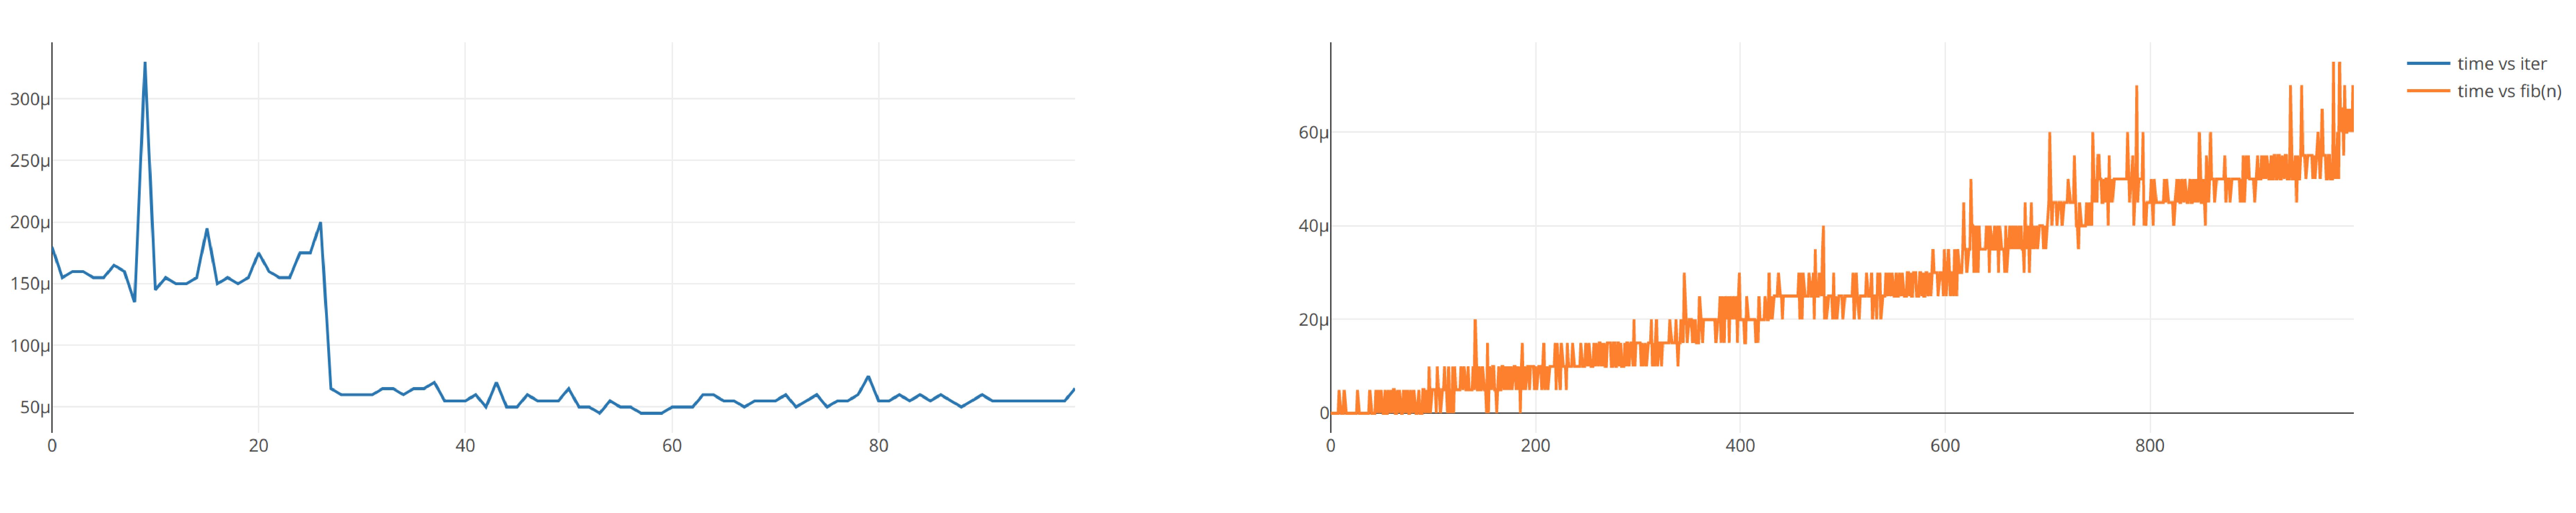
\includegraphics[width=\columnwidth]{figs/result.pdf}
      \caption{フィボナッチ数: CPU数ごとの比較}
      \label{figure:fib_cpu}
    \end{minipage}
  \end{center}
\end{figure}

\section{結論,考察}
実験1では,繰り返し実行を行うごとに、


%% \bibliographystyle{junsrt}
%% \bibliography{p-report}

\end{document}
